\documentclass[First Project.tex]{subfiles}

\begin{document}


\section{ Άσκηση 1 }
Στην \textbf{1η άσκηση} μας δίνεται αρχικά η συνάρτηση 
\begin{equation*}
    f(x) = e^{sin^{3}x} + x^{6} -2x^{4} -x^{3} -1
\end{equation*}
και ζητείται η γραφική παραστάση της στο διάστημα [-2,2].
\vspace{10px}
\begin{figure}[h!]
    \centering
    \captionsetup{justification=centering}
    \begin{center}
        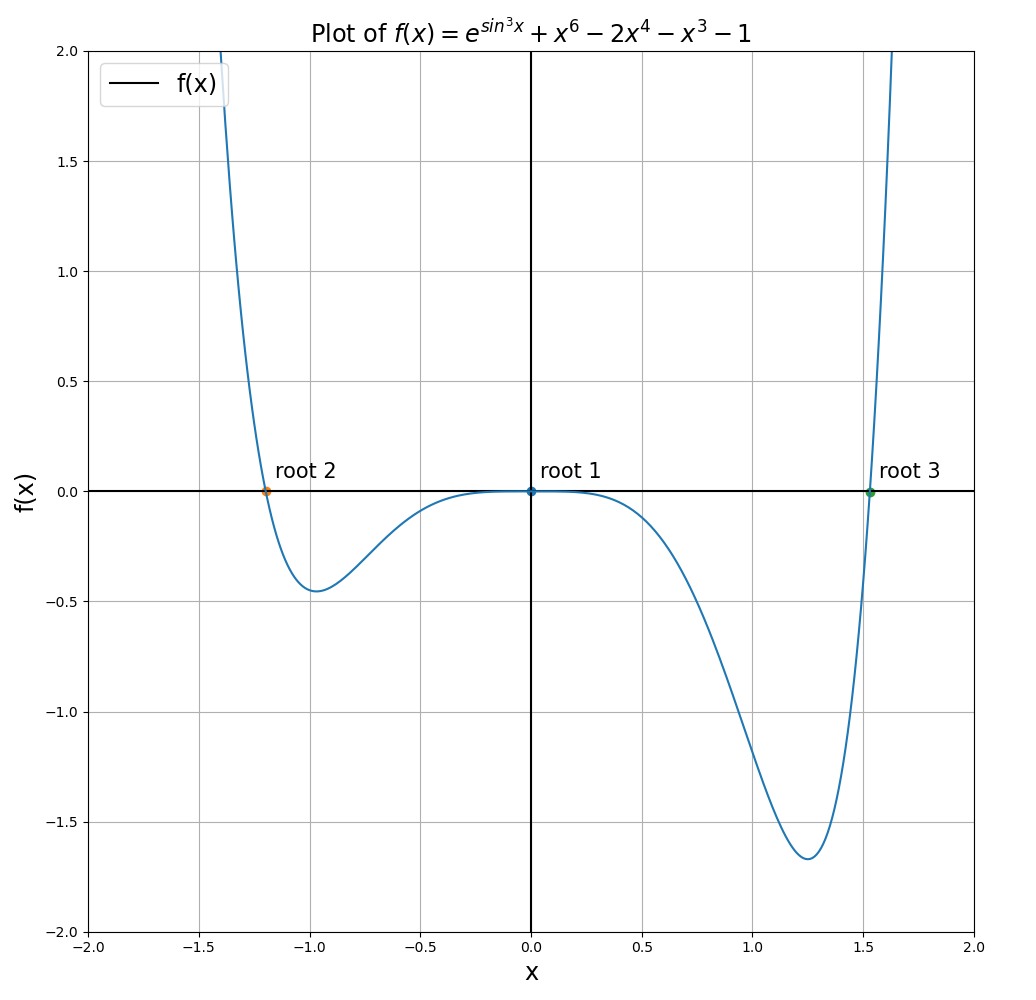
\includegraphics[scale=0.40]{exercise_1_function.png}    
        \caption{Γραφική παράσταση της συνάρτησης \textlatin{\textbf{f(x)}}}
    \end{center}
\end{figure}

Από την οποία παρατηρούμε στο \textit{Σχήμα 1} ότι η συνάρτηση έχει 3 ρίζες.Στην συνέχεια ζητείται να υπολογισθούν αυτές οι ρίζες με 
ακρίβεια 5ου δεκαδικού ψηφίου χρησιμοποιώντας την μέθοδο της διχοτόμησης, την μέθοδο \textlatin{Newton-Raphson} και τέλος την 
μέθοδος της τέμνουσας.


\end{document}